%
% This is an example LaTeX file which uses the SANDreport class file.
% It shows how a SAND report should be formatted, what sections and
% elements it should contain, and how to use the SANDreport class.
% It uses the LaTeX article class, but not the strict option.
% ItINLreport uses .eps logos and files to show how pdflatex can be used
%
% Get the latest version of the class file and more at
%    http://www.cs.sandia.gov/~rolf/SANDreport
%
% This file and the SANDreport.cls file are based on information
% contained in "Guide to Preparing {SAND} Reports", Sand98-0730, edited
% by Tamara K. Locke, and the newer "Guide to Preparing SAND Reports and
% Other Communication Products", SAND2002-2068P.
% Please send corrections and suggestions for improvements to
% Rolf Riesen, Org. 9223, MS 1110, rolf@cs.sandia.gov
%
\documentclass[pdf,12pt]{INLreport}
% pslatex is really old (1994).  It attempts to merge the times and mathptm packages.
% My opinion is that it produces a really bad looking math font.  So why are we using it?
% If you just want to change the text font, you should just \usepackage{times}.
% \usepackage{pslatex}
\usepackage{times}
\usepackage[FIGBOTCAP,normal,bf,tight]{subfigure}
\usepackage{amsmath}
\usepackage{amssymb}
\usepackage{soul}
\usepackage{pifont}
\usepackage{enumerate}
\usepackage{listings}
\usepackage{fullpage}
\usepackage{xcolor}          % Using xcolor for more robust color specification
\usepackage{ifthen}          % For simple checking in newcommand blocks
\usepackage{textcomp}
\usepackage{mathtools}
\usepackage{relsize}
\usepackage{lscape}
\usepackage[toc,page]{appendix}
\usepackage{RAVEN}

\newtheorem{mydef}{Definition}
\newcommand{\norm}[1]{\lVert#1\rVert}
%\usepackage[table,xcdraw]{xcolor}
%\usepackage{authblk}         % For making the author list look prettier
%\renewcommand\Authsep{,~\,}

% Custom colors
\definecolor{deepblue}{rgb}{0,0,0.5}
\definecolor{deepred}{rgb}{0.6,0,0}
\definecolor{deepgreen}{rgb}{0,0.5,0}
\definecolor{forestgreen}{RGB}{34,139,34}
\definecolor{orangered}{RGB}{239,134,64}
\definecolor{darkblue}{rgb}{0.0,0.0,0.6}
\definecolor{gray}{rgb}{0.4,0.4,0.4}

\lstset {
  basicstyle=\ttfamily,
  frame=single
}


\setcounter{secnumdepth}{5}
\lstdefinestyle{XML} {
    language=XML,
    extendedchars=true,
    breaklines=true,
    breakatwhitespace=true,
%    emph={name,dim,interactive,overwrite},
    emphstyle=\color{red},
    basicstyle=\ttfamily,
%    columns=fullflexible,
    commentstyle=\color{gray}\upshape,
    morestring=[b]",
    morecomment=[s]{<?}{?>},
    morecomment=[s][\color{forestgreen}]{<!--}{-->},
    keywordstyle=\color{cyan},
    stringstyle=\ttfamily\color{black},
    tagstyle=\color{darkblue}\bf\ttfamily,
    morekeywords={name,type},
%    morekeywords={name,attribute,source,variables,version,type,release,x,z,y,xlabel,ylabel,how,text,param1,param2,color,label},
}
\lstset{language=python,upquote=true}

\usepackage{titlesec}
\newcommand{\sectionbreak}{\clearpage}
\setcounter{secnumdepth}{4}

%\titleformat{\paragraph}
%{\normalfont\normalsize\bfseries}{\theparagraph}{1em}{}
%\titlespacing*{\paragraph}
%{0pt}{3.25ex plus 1ex minus .2ex}{1.5ex plus .2ex}

%%%%%%%% Begin comands definition to input python code into document
\usepackage[utf8]{inputenc}

% Default fixed font does not support bold face
\DeclareFixedFont{\ttb}{T1}{txtt}{bx}{n}{9} % for bold
\DeclareFixedFont{\ttm}{T1}{txtt}{m}{n}{9}  % for normal

\usepackage{listings}

% Python style for highlighting
\newcommand\pythonstyle{\lstset{
language=Python,
basicstyle=\ttm,
otherkeywords={self, none, return},             % Add keywords here
keywordstyle=\ttb\color{deepblue},
emph={MyClass,__init__},          % Custom highlighting
emphstyle=\ttb\color{deepred},    % Custom highlighting style
stringstyle=\color{deepgreen},
frame=tb,                         % Any extra options here
showstringspaces=false            %
}}


% Python environment
\lstnewenvironment{python}[1][]
{
\pythonstyle
\lstset{#1}
}
{}

% Python for external files
\newcommand\pythonexternal[2][]{{
\pythonstyle
\lstinputlisting[#1]{#2}}}

\lstnewenvironment{xml}
{}
{}

% Python for inline
\newcommand\pythoninline[1]{{\pythonstyle\lstinline!#1!}}

% Named Colors for the comments below (Attempted to match git symbol colors)
\definecolor{RScolor}{HTML}{8EB361}  % Sonat (adjusted for clarity)
\definecolor{DPMcolor}{HTML}{E28B8D} % Dan
\definecolor{JCcolor}{HTML}{82A8D9}  % Josh (adjusted for clarity)
\definecolor{AAcolor}{HTML}{8D7F44}  % Andrea
\definecolor{CRcolor}{HTML}{AC39CE}  % Cristian
\definecolor{RKcolor}{HTML}{3ECC8D}  % Bob (adjusted for clarity)
\definecolor{DMcolor}{HTML}{276605}  % Diego (adjusted for clarity)
\definecolor{PTcolor}{HTML}{990000}  % Paul

\def\DRAFT{} % Uncomment this if you want to see the notes people have been adding
% Comment command for developers (Should only be used under active development)
\ifdefined\DRAFT
  \newcommand{\nameLabeler}[3]{\textcolor{#2}{[[#1: #3]]}}
\else
  \newcommand{\nameLabeler}[3]{}
\fi
\newcommand{\alfoa}[1] {\nameLabeler{Andrea}{AAcolor}{#1}}
\newcommand{\cristr}[1] {\nameLabeler{Cristian}{CRcolor}{#1}}
\newcommand{\mandd}[1] {\nameLabeler{Diego}{DMcolor}{#1}}
\newcommand{\maljdan}[1] {\nameLabeler{Dan}{DPMcolor}{#1}}
\newcommand{\cogljj}[1] {\nameLabeler{Josh}{JCcolor}{#1}}
\newcommand{\bobk}[1] {\nameLabeler{Bob}{RKcolor}{#1}}
\newcommand{\senrs}[1] {\nameLabeler{Sonat}{RScolor}{#1}}
\newcommand{\talbpaul}[1] {\nameLabeler{Paul}{PTcolor}{#1}}
% Commands for making the LaTeX a bit more uniform and cleaner
\newcommand{\TODO}[1]    {\textcolor{red}{\textit{(#1)}}}
\newcommand{\xmlAttrRequired}[1] {\textcolor{red}{\textbf{\texttt{#1}}}}
\newcommand{\xmlAttr}[1] {\textcolor{cyan}{\textbf{\texttt{#1}}}}
\newcommand{\xmlNodeRequired}[1] {\textcolor{deepblue}{\textbf{\texttt{<#1>}}}}
\newcommand{\xmlNode}[1] {\textcolor{darkblue}{\textbf{\texttt{<#1>}}}}
\newcommand{\xmlString}[1] {\textcolor{black}{\textbf{\texttt{'#1'}}}}
\newcommand{\xmlDesc}[1] {\textbf{\textit{#1}}} % Maybe a misnomer, but I am
                                                % using this to detail the data
                                                % type and necessity of an XML
                                                % node or attribute,
                                                % xmlDesc = XML description
\newcommand{\default}[1]{~\\*\textit{Default: #1}}
\newcommand{\nb} {\textcolor{deepgreen}{\textbf{~Note:}}~}


%%%%%%%% End comands definition to input python code into document

%\usepackage[dvips,light,first,bottomafter]{draftcopy}
%\draftcopyName{Sample, contains no OUO}{70}
%\draftcopyName{Draft}{300}

% The bm package provides \bm for bold math fonts.  Apparently
% \boldsymbol, which I used to always use, is now considered
% obsolete.  Also, \boldsymbol doesn't even seem to work with
% the fonts used in this particular document...
\usepackage{bm}


% Define tensors to be in bold math font.
\newcommand{\tensor}[1]{{\bm{#1}}}

% Override the formatting used by \vec.  Instead of a little arrow
% over the letter, this creates a bold character.
\renewcommand{\vec}{\bm}

% Define unit vector notation.  If you don't override the
% behavior of \vec, you probably want to use the second one.
\newcommand{\unit}[1]{\hat{\bm{#1}}}
% \newcommand{\unit}[1]{\hat{#1}}

% Use this to refer to a single component of a unit vector.
\newcommand{\scalarunit}[1]{\hat{#1}}

% Aliases
\newcommand{\raven}{\texttt{RAVEN}}
\newcommand{\ravens}{\texttt{RAVEN}'s}
\newcommand{\plugin}{\raven{} Plugin}
\newcommand{\plugins}{\raven{} Plugins}


% \toprule, \midrule, \bottomrule for tables
\usepackage{booktabs}

% \llbracket, \rrbracket
\usepackage{stmaryrd}

\usepackage{hyperref}
\hypersetup{
    colorlinks,
    citecolor=black,
    filecolor=black,
    linkcolor=black,
    urlcolor=black
}

% Compress lists of citations like [33,34,35,36,37] to [33-37]
\usepackage{cite}

% If you want to relax some of the SAND98-0730 requirements, use the "relax"
% option. It adds spaces and boldface in the table of contents, and does not
% force the page layout sizes.
% e.g. \documentclass[relax,12pt]{SANDreport}
%
% You can also use the "strict" option, which applies even more of the
% SAND98-0730 guidelines. It gets rid of section numbers which are often
% useful; e.g. \documentclass[strict]{SANDreport}

% The INLreport class uses \flushbottom formatting by default (since
% it's intended to be two-sided document).  \flushbottom causes
% additional space to be inserted both before and after paragraphs so
% that no matter how much text is actually available, it fills up the
% page from top to bottom.  My feeling is that \raggedbottom looks much
% better, primarily because most people will view the report
% electronically and not in a two-sided printed format where some argue
% \raggedbottom looks worse.  If we really want to have the original
% behavior, we can comment out this line...
\raggedbottom
\setcounter{secnumdepth}{5} % show 5 levels of subsection
\setcounter{tocdepth}{5} % include 5 levels of subsection in table of contents

% ---------------------------------------------------------------------------- %
%
% Set the title, author, and date
%
\title{RAVEN Plugins Manual}
%\author{%
%\begin{tabular}{c} Author 1 \\ University1 \\ Mail1 \\ \\
%Author 3 \\ University3 \\ Mail3 \end{tabular} \and
%\begin{tabular}{c} Author 2 \\ University2 \\ Mail2 \\ \\
%Author 4 \\ University4 \\ Mail4\\
%\end{tabular} }


\author{ TODO authors
%\\Paul W. Talbot
%\\Andrea Alfonsi
%\\Cristian Rabiti
%\\Diego Mandelli
%\\Joshua Cogliati
%\\Congjian Wang
%\\Daniel P. Maljovec
%\\Curtis Smith
}
% \\James B. Tompkins}   Just people who actually ``developed'' a significant capability in the code should be placed here. Andrea
%\author{\textbf{\textit{Main Developers:}}  \\Andrea Alfonsi}
%\affil{Idaho National Laboratory, Idaho Falls, ID 83402}
%\\\{cristian.rabiti, andrea.alfonsi, joshua.cogliati, diego.mandelli, robert.kinoshita, ramazan.sen\}@inl.gov}

% There is a "Printed" date on the title page of a SAND report, so
% the generic \date should [WorkingDir:]generally be empty.
\date{}


% ---------------------------------------------------------------------------- %
% Set some things we need for SAND reports. These are mandatory
%
\SANDnum{INL/EXT-TODO}
\SANDprintDate{\today}
\SANDauthor{TODO authors} %Andrea Alfonsi, Cristian Rabiti, Diego Mandelli, Joshua Cogliati, Congjian Wang, Paul W. Talbot, Daniel P. Maljovec, Curtis Smith}
\SANDreleaseType{Revision 0}


% ---------------------------------------------------------------------------- %
% Include the markings required for your SAND report. The default is "Unlimited
% Release". You may have to edit the file included here, or create your own
% (see the examples provided).
%
% \include{MarkOUO} % Not needed for unlimted release reports

\def\component#1{\texttt{#1}}

% ---------------------------------------------------------------------------- %
\newcommand{\systemtau}{\tensor{\tau}_{\!\text{SUPG}}}

% Added by Sonat
\usepackage{placeins}
\usepackage{array}

\newcolumntype{L}[1]{>{\raggedright\let\newline\\\arraybackslash\hspace{0pt}}m{#1}}
\newcolumntype{C}[1]{>{\centering\let\newline\\\arraybackslash\hspace{0pt}}m{#1}}
\newcolumntype{R}[1]{>{\raggedleft\let\newline\\\arraybackslash\hspace{0pt}}m{#1}}

% end added by Sonat
% ---------------------------------------------------------------------------- %
%
% Start the document
%

\begin{document}

    \maketitle

    % ------------------------------------------------------------------------ %
    % An Abstract is required for SAND reports
    %
%    \begin{abstract}
%    \input abstract
%    \end{abstract}


    % ------------------------------------------------------------------------ %
    % An Acknowledgement section is optional but important, if someone made
    % contributions or helped beyond the normal part of a work assignment.
    % Use \section* since we don't want it in the table of context
    %
%    \clearpage
%    \section*{Acknowledgment}



%	The format of this report is based on information found
%	in~\cite{Sand98-0730}.


    % ------------------------------------------------------------------------ %
    % The table of contents and list of figures and tables
    % Comment out \listoffigures and \listoftables if there are no
    % figures or tables. Make sure this starts on an odd numbered page
    %
    \cleardoublepage		% TOC needs to start on an odd page
    \tableofcontents
    %\listoffigures
    %\listoftables


    % ---------------------------------------------------------------------- %
    % An optional preface or Foreword
%    \clearpage
%    \section*{Preface}
%    \addcontentsline{toc}{section}{Preface}
%	Although muggles usually have only limited experience with
%	magic, and many even dispute its existence, it is worthwhile
%	to be open minded and explore the possibilities.


    % ---------------------------------------------------------------------- %
    % An optional executive summary
    %\clearpage
    %\section*{Summary}
    %\addcontentsline{toc}{section}{Summary}
    %\input{Summary.tex}
%	Once a certain level of mistrust and skepticism has
%	been overcome, magic finds many uses in todays science



%	and engineering. In this report we explain some of the
%	fundamental spells and instruments of magic and wizardry. We
%	then conclude with a few examples on how they can be used
%	in daily activities at national Laboratories.


    % ---------------------------------------------------------------------- %
    % An optional glossary. We don't want it to be numbered
%    \clearpage
%    \section*{Nomenclature}
%    \addcontentsline{toc}{section}{Nomenclature}
%    \begin{description}
%          \item[alohomoral]
%           spell to open locked doors and containers
%          \item[leviosa]
%           spell to levitate objects
%    \item[remembrall]
%           device to alert you that you have forgotten something
%    \item[wand]
%           device to execute spells
%    \end{description}


    % ---------------------------------------------------------------------- %
    % This is where the body of the report begins; usually with an Introduction
    %
    \SANDmain		% Start the main part of the report

\section{Introduction}

RAVEN (Risk Analysis Virtual ENvironment) [TODO cite] is a powerful tool for risk- and uncertainty-based stochastic analysis. TODO say more.

Occasionally, the applications of RAVEN become sufficiently varied and complex to warrant a special application to a particular suite of problems. These special applications may introduce new physics, new templates, new RAVEN entities, or any combination of the above. In this instance, it's worth considering whether developing a Plugin could be beneficial to you and the community.

\subsection{What are Plugins?}

Plugins are defined the RAVEN Software Quality Assurance documentation [TODO CITE]. They are intended to allow development that does not fit in the scope of RAVENs mission to be completed in a way that is still captured under the umbrella of RAVEN-based tools.

\subsection{What isn't a Plugin?}

While Plugins have wide applicability to extending the functionaliy of RAVEN, there are some alternatives that may be more suitable for some developments.

A Plugin is not simple a RAVEN Template. RAVEN Templates are used to simplify complex RAVEN workflows for more restrictive but increasingly efficient workflow permutations. If the end result of development is only a new RAVEN Template, we recommend you contribute this as a new templated workflow rather than a separate Plugin.

A Plugin is not a set of models that do similar activities to what RAVEN already does. For example, if new development includes RAVEN postprocessors and RAVEN metrics for uncertainty analysis and clustering using a particular theory, this is well within RAVENs scope and should be directly contributed to the code so these additions can benefit the community directly without the Plugin interaction.

\subsection{How do I decide?}

Ultimately, the decision to develop a plugin is best discussed with the RAVEN core team. However, the following guidelines may help inform a good decision.

\begin{figure}[h!]
  \centering
  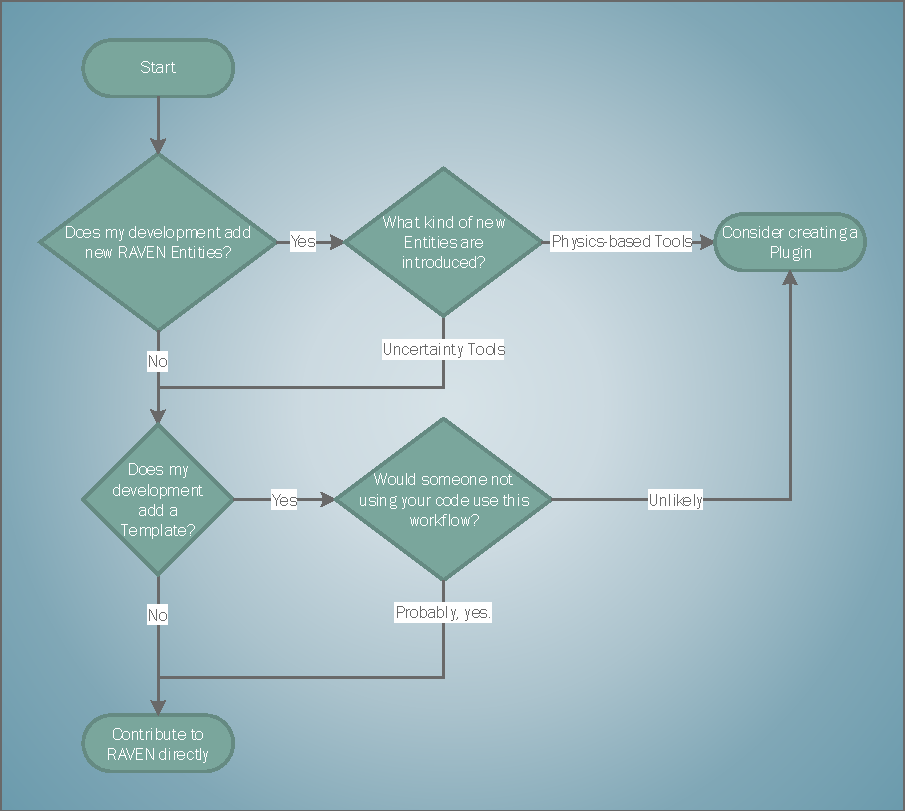
\includegraphics[scale=0.7]{pics/toPluginOrNot.pdf}
  \caption{Choosing to Plugin Workflow}
  \label{fig:choose plugin}
 \end{figure}

 \subsection{Supported Plugins}

 Officially supported RAVEN Plugins are a subset of all Plugins filtered by a particular set of characteristics. It is intended that all official Plugins are compatible with the latest developments in RAVEN as well as with each other. Additionally, official plugins contain continuous integration (CI) testing and provide the necessary software quality assurance (SQA) documentation to be included in RAVEN's SQA plan.

 To be an officially supported RAVEN Plugin, the following prerequesites must be met:
 \begin{itemize}
  \item The appropriate SQA documentation for NQA-1 level 2 coverage under the RAVEN SQA must be in place for the Plugin.
  \item The Plugin must contain CI testing with coverage consistent with RAVEN SQA. This CI testing must be compatible with RAVEN's CI testing system.
  \item The Plugin must contain documentation explaining the use and options included in the Plugin's contents.
  \item If at any time a change in RAVEN causes a failure in the CI tests in the plugin, the plugin must be updated to be compatible with the new RAVEN.
 \end{itemize}

 If a Plugin fails any of these criteria, a grace period (usually a month) is provided along with notification to the Plugin developers. If the grace period expires and the Plugin does not meet the requirements, it may be removed from the official supported Plugins list, pending an update to the Plugin.
% \section{Introduction}

RAVEN (Risk Analysis Virtual ENvironment) [TODO cite] is a powerful tool for risk- and uncertainty-based stochastic analysis. TODO say more.

Occasionally, the applications of RAVEN become sufficiently varied and complex to warrant a special application to a particular suite of problems. These special applications may introduce new physics, new templates, new RAVEN entities, or any combination of the above. In this instance, it's worth considering whether developing a Plugin could be beneficial to you and the community.

\subsection{What are Plugins?}

Plugins are defined the RAVEN Software Quality Assurance documentation [TODO CITE]. They are intended to allow development that does not fit in the scope of RAVENs mission to be completed in a way that is still captured under the umbrella of RAVEN-based tools.

\subsection{What isn't a Plugin?}

While Plugins have wide applicability to extending the functionaliy of RAVEN, there are some alternatives that may be more suitable for some developments.

A Plugin is not simple a RAVEN Template. RAVEN Templates are used to simplify complex RAVEN workflows for more restrictive but increasingly efficient workflow permutations. If the end result of development is only a new RAVEN Template, we recommend you contribute this as a new templated workflow rather than a separate Plugin.

A Plugin is not a set of models that do similar activities to what RAVEN already does. For example, if new development includes RAVEN postprocessors and RAVEN metrics for uncertainty analysis and clustering using a particular theory, this is well within RAVENs scope and should be directly contributed to the code so these additions can benefit the community directly without the Plugin interaction.

\subsection{How do I decide?}

Ultimately, the decision to develop a plugin is best discussed with the RAVEN core team. However, the following guidelines may help inform a good decision.

\begin{figure}[h!]
  \centering
  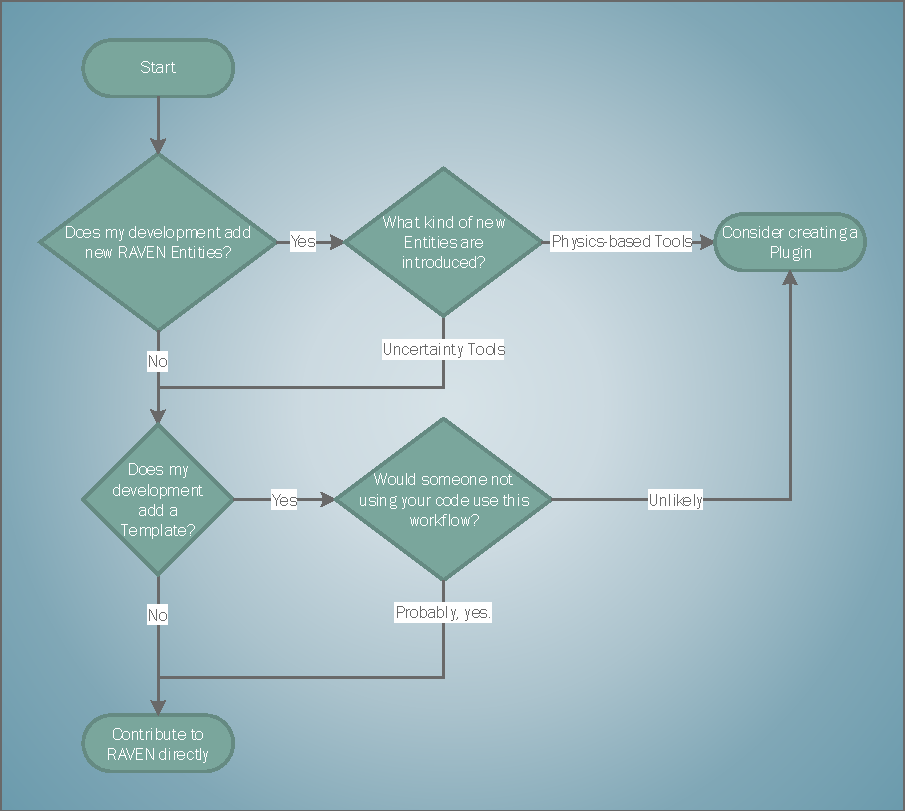
\includegraphics[scale=0.7]{pics/toPluginOrNot.pdf}
  \caption{Choosing to Plugin Workflow}
  \label{fig:choose plugin}
 \end{figure}

 \subsection{Supported Plugins}

 Officially supported RAVEN Plugins are a subset of all Plugins filtered by a particular set of characteristics. It is intended that all official Plugins are compatible with the latest developments in RAVEN as well as with each other. Additionally, official plugins contain continuous integration (CI) testing and provide the necessary software quality assurance (SQA) documentation to be included in RAVEN's SQA plan.

 To be an officially supported RAVEN Plugin, the following prerequesites must be met:
 \begin{itemize}
  \item The appropriate SQA documentation for NQA-1 level 2 coverage under the RAVEN SQA must be in place for the Plugin.
  \item The Plugin must contain CI testing with coverage consistent with RAVEN SQA. This CI testing must be compatible with RAVEN's CI testing system.
  \item The Plugin must contain documentation explaining the use and options included in the Plugin's contents.
  \item If at any time a change in RAVEN causes a failure in the CI tests in the plugin, the plugin must be updated to be compatible with the new RAVEN.
 \end{itemize}

 If a Plugin fails any of these criteria, a grace period (usually a month) is provided along with notification to the Plugin developers. If the grace period expires and the Plugin does not meet the requirements, it may be removed from the official supported Plugins list, pending an update to the Plugin.


\clearpage
\begin{appendices}
  \section{Document Version Information}
  \input{../version.tex}
\end{appendices}
%\input{examplesPrimer.tex}


    % ---------------------------------------------------------------------- %
    % References
    %
    \clearpage
    % If hyperref is included, then \phantomsection is already defined.
    % If not, we need to define it.
    \providecommand*{\phantomsection}{}
    \phantomsection
    \addcontentsline{toc}{section}{References}
    % \bibliographystyle{ieeetr}
    % \bibliography{raven_theory_manual}


    % ---------------------------------------------------------------------- %
    %

    % \printindex

    %\include{distribution}

\end{document}
